\documentclass[12pt]{amsart}
\usepackage{ytableau,graphicx, xypic}
\xyoption{all}
\title{An Introduction to Schur Functions}
\author{Amritanshu Prasad}
\newtheorem{theorem}{Theorem}[subsection]
\newtheorem{lemma}[theorem]{Lemma}
\newtheorem{corollary}[theorem]{Corollary}
\theoremstyle{definition}
\newtheorem{definition}[theorem]{Definition}
\theoremstyle{example}
\newtheorem{example}[theorem]{Example}
\newtheorem{exercise}[theorem]{Exercise}
\begin{document}
\maketitle
\renewcommand{\thesubsection}{\arabic{subsection}}
\subsection{Symmetric Functions}
\label{sec:symmetric-functions}
We consider polynomials in $n$ variables $x_1,\dotsc,x_n$.
Given a multiindex $\alpha=(\alpha_1,\dotsc, \alpha_n)$, $x^\alpha$ denotes the monomial $x_1^{\alpha_1}\dotsb x_n^{\alpha_n}$
A symmetric polynomial in $n$ variables $x_1,\dotsc, x_n$ is a polynomial of the form
\begin{displaymath}
  f(x_1,\dotsc, x_n) = \sum_{\alpha} c_\alpha x^\alpha,
\end{displaymath}
where, for any permutation $w\in S_n$,
\begin{displaymath}
  c_{(\alpha_1,\dotsc,\alpha_n)} = c_{(\alpha_{w(1)},\dotsc,\alpha_{w(n)})}.
\end{displaymath}
We call the integer partition $\lambda$ obtained by sorting the coordinates of $\alpha$ the shape of $\alpha$ and write $\lambda = \lambda(\alpha)$.
The most obvious example of a symmetric polynomial in $n$ variables is the \emph{monomial symmetric function}, defined for each integer partition $\lambda$:
\begin{displaymath}
  m_\lambda = \sum_{\lambda(\alpha) = \lambda} c_\alpha x^\alpha.
\end{displaymath}
Note that $m_\lambda$ is homogeneous of degree $|\lambda|$ (the sum of the parts of $\lambda$).
\begin{exercise}
  Take $n=4$. Compute the monomial symmetric functions $m_{(3)}$, $m_{(2,1)}$, and $m_{(1^3)}$.
\end{exercise}
\begin{theorem}
The polynomials $m_\lambda(x_1,\dotsc,x_n)$, as $\lambda$ runs over all the integer partition of $d$, form a basis for the space of homogeneous symmetric polynomials of degree $d$ in $n$ variables.
\end{theorem}
\subsection{Complete and Elementary Symmetric Polynomials}
\label{sec:compl-elem-symm}
Recall that the coefficients of a polynomial are symmetric polynomials in its roots:
\begin{multline}
  \label{eq:elem-id}
  (t-x_1)(t-x_2)\dotsb (t-x_n) \\= t^n - e_1(x_1,\dotsc, x_n)t^{n-1} + \dotsb + (-1)^n e_n(x_1,\dotsc, x_n),
\end{multline}
where coefficient $e_i(x_1,\dotsc, x_n)$ of $t^{n-i}$ is given by:
\begin{equation}
  \label{eq:elem}
  e_i(x_1,\dotsc, x_n) = \sum_{1\leq j_1<\dotsb<j_i\leq n} x_{j_1}x_{j_2}\dotsb x_{j_i}.
\end{equation}
The polynomial $e_i$ is called the $i$th \emph{elementary symmetric polynomial}.
By convention, write $e_i(x_1,\dotsc,x_n)=0$, for $i>n$.

The identity (\ref{eq:elem-id}) can be written more elegantly as:
\begin{displaymath}
  (1+t x_1) \dotsb (1+tx_n) = \sum_{i=0}^n e_i(x_1,\dotsb, x_n)t^i.
\end{displaymath}

Dually\footnote{We will refer to the replacing of $(1+u)$ by $(1-u)^{-1}$ in a formal identity as \emph{dualization}.}, the \emph{complete symmetric polynomials} are defined by the formal identity:
\begin{displaymath}
  \frac 1{(1-x_1t)\dotsb (1-x_nt)} = \sum_{i=0}^\infty h_i(x_1,\dotsb, x_n)t^i.
\end{displaymath}
\begin{example}
  In three variables, we have:
  \begin{align*}
    e_2(x_1,x_2,x_3) & = x_1x_2 + x_1x_3 + x_2x_3,\\
    h_2(x_1,x_2,x_3) & = x_1^2 + x_1x_2 + x_1x_3 + x_2^2 + x_2x_3 + x_2^3.
  \end{align*}
\end{example}
\begin{exercise}
  Show that
  \begin{displaymath}
    h_i(x_1,\dotsb x_n) = \sum_{1\leq j_1\leq \dotsb \leq j_i\leq n} x_{j_1}\dotsb x_{j_i}.
  \end{displaymath}
\end{exercise}
More generally, for any integer partition $\lambda=(\lambda_1,\dotsc, \lambda_l)$, define:
\begin{align*}
  h_\lambda &= h_{\lambda_1} h_{\lambda_2}\dotsb h_{\lambda_l},\\
  e_\lambda &= e_{\lambda_1} e_{\lambda_2}\dotsb e_{\lambda_l}.
\end{align*}
\begin{theorem}
  Given integer partitions $\lambda=(\lambda_1,\dotsc,\lambda_l)$ and $\mu=(\mu_1,\dotsb, \mu_m)$ of and integer $d$, let $M_{\lambda\mu}$ denote the number of integer matrices $(a_{ij})$ with non-negative entries whose $i$th row sums to $\lambda_i$ for each $i$, and whose $j$th column sums to $\mu_j$ for each $j$.
  Then
  \begin{displaymath}
    h_\lambda = \sum_\mu M_{\lambda\mu} m_\mu.
  \end{displaymath}
  Dually, let $=N_{\lambda\mu}$ denote the number of integer matrices $(a_{ij})$ with entries $0$ or $1$, whose $i$th row sums to $\lambda_i$ for each $i$, and whose $j$th column sums to $\mu_j$ for each $j$.
  \begin{displaymath}
    e_\lambda = \sum_\mu N_{\lambda\mu} m_\mu.
  \end{displaymath}
\end{theorem}
\begin{proof}
  We first prove the second identity involving elementary symmetric functions.
  A monomial in the expansion:
  \begin{displaymath}
    e_\lambda = \prod_{i=1}^l \sum_{j_1<\dotsb<j_{\lambda_j}}x_{j_1}\dotsb x_{j_{\lambda_i}}
  \end{displaymath}
  is a product of summands, one chosen from each of the $l$ factors.
  Construct an $l\times m$ matrix $(a_{ij})$ corresponding to such a choice as follows:
  if the summand $x_{j_1}\dotsb x_{j_{\lambda_i}}$ is chosen from the $i$th factor, then set the entries $a_{i,j_1},\dotsc, a_{i, j_{\lambda_j}}$ to be $1$ (the remaining entries of the $i$th row are $0$).
  Clearly the $i$th row of such a matrix sums to $\lambda_i$.
  The monomial corresponding to this choice is $x^\mu$ if, for each $j$, the the number of $i$ for which $x_j$ appears in $a_{i,j_1},\dotsc, a_{i, j_{\lambda_j}}$, which is the sum of the $j$th column of the matrix $(a_{ij})$.
  It follows that the coefficient of $x^\mu$, and hence the coefficient of $m_\mu$ in the expansion of $e_\lambda$ in the basis of monomial symmetric functions of degree $n$, is $N_{\lambda\mu}$.

A similar proof can be given for the first identity involving complete symmetric functions. The only difference is that a variables are repeated in the monomials that appear in $h_i$. Counting the number of repetitions (instead of just recording $0$ or $1$) gives non-negative integer matrices.
\end{proof}
\subsection{Alternating Polynomials}
\label{sec:alt-poly}
An \emph{alternating polynomial} in $x_1,\dotsc, x_n$ is of the form:
\begin{equation}
  \label{eq:alt-form}
  f(x_1,\dotsc,x_n) = \sum_{\alpha} c_\alpha x_\alpha,
\end{equation}
where, $c_{w(\alpha)} = \epsilon(w)c_\alpha$ for every multiindex $\alpha$ as in Section~\ref{sec:symmetric-functions}.
Here $\epsilon:S_n\to \{\pm 1\}$ denotes the sign function.
Equivalently, an alternating polynomial is one whose sign is reversed upon the interchange of any two variables.
\begin{exercise}
  If $\alpha$ is a multiindex where $\alpha_i=\alpha_j$ for some $i\neq j$, then $c_\alpha = 0$.
\end{exercise}
In particular, every monomial in an alternating polynomial must be composed of distinct powers.
Moreover, the polynomial is completely determined by the coefficients $c_\alpha$ of strictly decreasing multiindices, namely, multiindices of the form $\alpha=(\alpha_1,\dotsc,\alpha_n)$ with $\alpha_1>\dotsb>\alpha_n$.
\begin{exercise}
  Let $\delta$ denote the strictly increasing multiindex $(n-1,n-2,\dotsc,1, 0)$ of lowest degree.
  Given an integer partition with at most $n$ parts, we will pad it with $0$'s so that it can be regarded as a weakly decreasing multiindex.
  Then $\lambda\mapsto \lambda+\delta$ is a bijection from the set of integer partitions with at most $n$ onto the set of strictly decreasing multiindices.
\end{exercise}
\begin{example}
  Let $\lambda = (\lambda_1,\dotsc, \lambda_n)$ be a weakly decreasing multiindex.
  The polynomial:
  \begin{displaymath}
    a_{\lambda+\delta} = \det(x_i^{\lambda_j + n - j})
  \end{displaymath}
  is alternating, with unique strictly decreasing monomial $x^{\lambda+\delta}$.
\end{example}
\begin{exercise}
  \label{exercise:alt-basis}
  The alternating polynomial of the form \textup{(\ref{eq:alt-form})} is equal to  \begin{displaymath}
    \sum_{\lambda} c_\lambda a_{\lambda+\delta},
  \end{displaymath}
  the sum being over all weakly decreasing multiindices.
\end{exercise}
\subsection{Cauchy's bialternant form of a Schur function}
\label{sec:cauchys-bialt-form}
The simplest polynomial of the form $a_{\lambda+\delta}$ arises when $\lambda=0$; $a_\delta$ is the Vandermonde determinant:
\begin{displaymath}
  a_\delta = \prod_{1\leq i<j\leq n}(x_i-x_j).
\end{displaymath}
\begin{exercise}
  Show that, for every weakly decreasing multiindex $\lambda$, $a_{\lambda+\delta}$ is divisible by $a_\delta$ in the ring of polynomials in $x_1,\dotsc,x_n$.
\end{exercise}
\begin{exercise}
  \label{exercise:vandermonde-iso}
  Show that $f\mapsto fa_\delta$ is an isomorphism of the space of symmetric polynomials in $x_1,\dotsc, x_n$ of degree $d$ onto the space of alternating polynomials of degree $d + \binom n2$.
\end{exercise}
The above exercise allows us to give the historically oldest definition of Schur functions---\emph{Cauchy's bialternant formula}:
\begin{equation}
  \label{eq:schur}
  s_\lambda(x_1,\dotsc,x_n) = a_{\lambda+\delta}/a_\delta,
\end{equation}
for any partition $\lambda$ with at most $n$ parts.
If $\lambda$ has more than $n$ parts, set $s_\lambda(x_1,\dotsc,x_n) =0$.
This is clearly a symmetric function of degree $|\lambda|$.
When $\lambda$ has more than $n$ parts, we shall write $s_\lambda(x_1,\dotsc,x_n)=0$
\begin{theorem}
  As $\lambda$ runs over all integer partitions of $d$ with at most $n$ parts, the Schur functions $s_\lambda(x_1,\dotsc,x_n)$ form a basis of the space of all homogeneous symmetric functions in $x_1,\dotsc,x_n$ of degree $d$.
\end{theorem}
\begin{proof}
  This follows from Exercises~\ref{exercise:alt-basis} and~\ref{exercise:vandermonde-iso}.
\end{proof}
\begin{exercise}
  [Stability of Schur functions]
  Show that substituting $x_n=0$ in the Schur function $s_\lambda(x_1,\dotsc, x_n)$ with $n$ variables gives the corresponding Schur function $s_\lambda(x_1,\dotsc,x_{n-1})$ with $n-1$ variables.
\end{exercise}
\subsection{Pieri's rule}
\label{sec:pieri}
The set of integer partitions is endowed with the \emph{containment order}.
We say that a partition $\lambda=(\lambda_1,\dotsc,\lambda_l)$ \emph{contains} a partition $\mu=(\mu_1,\dotsc, \mu_m)$ if $l \geq m$, and $\lambda_i\geq \mu_i$ for every $i=1,\dotsb, m$.
We write $\lambda\supset\mu$ or $\mu \subset \lambda$.
Recall that the Young diagram of the partition $\lambda$ is the set of points 
\begin{displaymath}
\{(i, j)\mid 1\leq i\leq l,\; 1\leq j\leq \lambda_i\}.
\end{displaymath}
Visually, each node $(i,j)$ of the Young diagram is replaced by a box, and the box corresponding to $(i,j)$ is placed in the $i$th row and $j$th column (matrix notation).
Thus, the Young diagram of $\lambda=(6, 5, 3, 3)$ is depicetd by:
\begin{displaymath}
  \ydiagram{6,5,3,3}
\end{displaymath}
Note that containment of partitions is nothing but the containment relation on their Young diagrams.
By abuse of notation, we will also use $\lambda$ to denote the Young diagram of $\lambda$.

By a skew-shape, we mean a difference of Young diagrams $\lambda \setminus \mu$, where $\lambda \supset \mu$.
We write $\lambda/\mu$ for this skew-shape.
A skew-shape is called a \emph{horizontal strip} (respectively, a \emph{vertical strip}) if it has at most one element in each vertical column (respectively, horizontal row).

\begin{theorem}
  For every partition $\lambda$, and every positive integer $k$,
  \begin{displaymath}
    s_\lambda h_k = \sum_\mu s_\mu,
  \end{displaymath}
  where the sum runs over all partitions $\mu\supset\lambda$ such that $\mu/\lambda$ is a horizontal strip of size $k$.
  Dually,
  \begin{displaymath}
    s_\lambda e_k = \sum_\mu s_\mu,
  \end{displaymath}
  where the sum runs over all partitions $\mu\supset\lambda$ such that $\mu/\lambda$ is a vertical strip of size $k$.
\end{theorem}
\begin{proof}
  The first identity is equivalent to showing that:
  \begin{displaymath}
    a_{\lambda+\delta} \sum_{\alpha_1+\dotsb+\alpha_n=k} x_1^{\alpha_1}\dotsb x_n^{\alpha_n} = \sum_\mu a_{\mu+\delta},
  \end{displaymath}
  the sum on the right being over all partitions $\mu\supset\lambda$ such that $\mu/\lambda$ is a horizontal strip.

  Writing $\alpha=(\alpha_1,\dotsc,\alpha_n)$, the sum on the left hand side can be regarded as a sum of determinants:
  \begin{equation}
    \label{eq:pieri-canc}
    a_{\lambda+\delta} \sum_{|\alpha|=k} x_1^{\alpha_1}\dotsb x_n^{\alpha_n} = \sum_{|\alpha|=k} a_{\lambda + \alpha + \delta}.
  \end{equation}
  Suppose there exists an integer $\alpha_i$ such that $\alpha_i>\lambda_i-\lambda_{i+1}$ (in other words, $(\lambda + \alpha)/\lambda$ is not a horizontal strip), then define $\beta=(\beta_1,\dotsc,\beta_n)$ by $\beta_i = \alpha_{i+1} - (\lambda_i - \lambda_{i+1} + 1)$, $\beta_{i+1} = \alpha_i + (\lambda_i - \lambda_{i+1} +1)$, and $\beta_j=\alpha_j$ for all $j\notin \{i, i+1\}$.
  Then $a_{\lambda+\alpha+\delta} = -a_{\lambda+\beta+\delta}$.
  So the only terms that survive on the right hand side of (\ref{eq:pieri-canc}) are of the form $a_{\mu+\delta}$, where $\mu/\lambda$ is a horizontal strip.

  The proof of the second identity in the theorem is similar (in fact, a little simpler) and is left to the reader as an exercise.
\end{proof}
As a special case of Pieri's rule, we have:
\begin{corollary}
  For every positive integer $k$,
  \begin{displaymath}
    s_{(k)} = h_k, \text{ and } s_{(1^k)} = e_k.
  \end{displaymath}
\end{corollary}
\subsection{Schur to Complete and Elementary via Tableaux}
Pieri's rule allows us to compute the complete and elementary symmetric functions $h_\lambda$ and $e_\lambda$ in terms of Schur functions.
\begin{example}
  Repeated application of Pieri's rule gives,:
  \begin{displaymath}
    e_{(2, 2, 1)} = 
    \xymatrix@R-1pc{
     &&&&e_2 e_2 e_1\ar[d]&&\\
    &&&&s_{(1^2)} e_2 e_1\ar[dll]\ar[d]\ar[dr]&&\\
    &&s_{(2^2)}e_1\ar[dll]\ar[dl] \ar[d]&& s_{(2, 1^2)}e_1\ar[dl]\ar[d]\ar[dr] & s_{(1^4)}e_1 \ar[dr]\ar[drr]&&\\
    s_{(3, 2)} & s_{(2^2, 1)} & s_{(3, 1^2)} & s_{(2^2, 1)} & s_{(2, 1^3)}] & s_{(2, 1^3)} & s_{(1^5)}
    }
  \end{displaymath}
  The steps going from the first line of the above calculation to each term of the last line can be recorded by putting numbers into Young diagrams:
  \begin{displaymath}
    \ytableaushort{113,22},
  \end{displaymath}
\end{example}
\subsection{The Lindstr\"om-Gessel-Viennot Lemma}
\label{sec:lgv}
Let $R$ be a commutative ring.
Let $S$ be any set of points, and $v:S\times S\to R$ be any function (we think of $w$ as a \emph{weight function}.
Given $s, t\in S$, a path in $S$ from $s$ to $t$ is is a sequence $\omega=(s=s_0,s_1,\dotsc,s_k=t)$ of distinct points in $S$.
We denote this by $\omega:s\to t$.
The weight of the path $\omega$ is defined to be:
\begin{displaymath}
  v(\omega) = v(s_0,s_1)v(s_1,s_2)\dotsb v(s_{k-1}, s_k).
\end{displaymath}
\begin{definition}
  [non-crossing paths]
  Two paths $\omega=(s_0,\dotsc, s_k)$ and $\eta=(t_0,\dotsc,t_l)$ are said to be non-crossing if $s_i\neq t_j$ for all $0\leq i \leq k$ and $0\leq t \leq l$.
\end{definition}
Fix points $A_1,\dotsc, A_n$ and $B_1,\dotsc, B_n$ in $S$, and define an $n\times n$ matrix $(a_{ij})$ by:
\begin{displaymath}
  a_{ij} = \sum_{\omega:A_i\to B_j} v(\omega).
\end{displaymath}
\begin{theorem}
  [Lindstr\"om-Gessel-Viennot Lemma]
  \label{lemma:lgv}
  The determinant of the matrix $(a_{ij})$ defined above is given by:
  \begin{displaymath}
    \det(a_{ij}) = \sum_{\omega_i:A_i\to B_i} v(\omega_1)\dotsb v(\omega_n),
  \end{displaymath}
  where the sum is over all $n$-tuples $(\omega_1,\dotsc, \omega_n)$ of pairwise non-crossing paths.
\end{theorem}
\subsection{The Jacobi-Trudi Identities}
\label{sec:jacobi-trudi-ident}
\begin{displaymath}
  s_\lambda = \det(h_{\lambda_i-i+j}), \quad s_{\lambda'} = \det(e_{\lambda_i-i+j}).
\end{displaymath}

For the first Jacobi-Trudi identity take $S$ to be the positive cone in the the integer lattice:
\begin{displaymath}
  S = \{(i,j)\mid i\geq 0,\; j>0 \text{ are integers}\}.
\end{displaymath}
Set the weight $v((i,j), (i+1,j))$ of each rightward horizontal edge to be $x_j$ for $j=1,\dotsc, n$, the weight of each downward vertical edge $v((i,j), (i,j-1))$ to be $1$ for all $j=2,\dotsc,n$.
The remaining weights are all zero.
\begin{lemma}
  \label{lemma:entry}
  For all integers $i>0$ and $j\geq 0$, we have:
  \begin{displaymath}
    \sum_{\omega:(i, n)\to (i+j, 1)} v(\omega) = h_j(x_1,\dotsc,x_n).
  \end{displaymath}
\end{lemma}
\begin{proof}
  Only rightward or downward steps have non-zero weights.
  So every path with non-zero weight is composed of unit downward and rightward steps.
  A path with non-zero weight from $(i, n)$ to $(i+j, 1)$ must have exactly $j$ rightward steps, say in rows $n\geq i_1\geq i_2 \dotsb \geq i_j\geq 1$.
  The weight of such a path is $x_{i_1}\dotsb x_{i_j}$, and hence, the sum of the weights of all such paths is $h_j(x_1,\dotsc, x_n)$. For an example, see Fig.~\ref{fig:path_example}.
\end{proof}
\begin{figure}
  \centering
  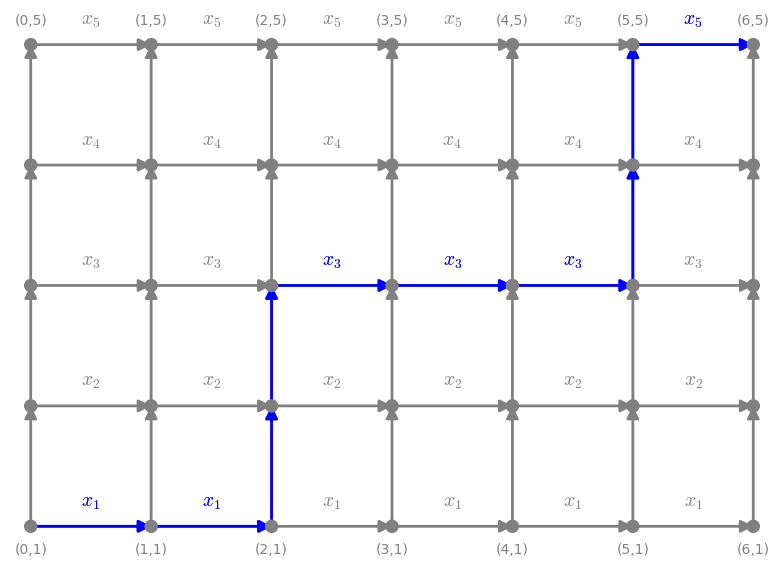
\includegraphics[width=\textwidth]{path_example.png}
  \caption{A path from $(0, 5)$ to $(6, 1)$ representing the monomial $x_1x_3^3x_5^2$ in $h_6$.}
  \label{fig:path_example}
\end{figure}
Let $A_i = (n-i, n)$ and $B_i=(\lambda_i+n-i, 1)$ for $i=1,\dotsc, n$.
Then  by Lemma~\ref{lemma:entry},
\begin{displaymath}
  \sum_{\omega:A_i\to B_j} v(\omega) = h_{\lambda_j+i-j}.
\end{displaymath}
\end{document}
